\documentclass[conference]{IEEEtran}
%\IEEEoverridecommandlockouts
% The preceding line is only needed to identify funding in the first footnote. If that is unneeded, please comment it out.
\usepackage{cite}
\usepackage{amsmath,amssymb,amsfonts}
\usepackage{algorithmic}
\usepackage{graphicx}
\usepackage{textcomp}
\usepackage{xcolor}
\def\BibTeX{{\rm B\kern-.05em{\sc i\kern-.025em b}\kern-.08em
    T\kern-.1667em\lower.7ex\hbox{E}\kern-.125emX}}
\begin{document}

\title{3-Bit Flash ADC \\
}

\author{\IEEEauthorblockN{Nicholas Snyder}
\IEEEauthorblockA{\textit{Department of Electrical and Computer Engineering} \\
\textit{University of New Hampshire}\\
Durham, United States of America \\
Nick.Snyder@usnh.edu}
}

\maketitle

\begin{abstract}
A 3-Bit Flash ADC was created using Cadense Virtuoso for the ECE 715 final project. It was made from custom designed logic gates and each different gate used was made into a layout that chip manufacturers can use to fabricate integrated circuits. Each layout was tested against Cadense's DRC, LVS, and QRC testing suites to ensure design accuracy.
\end{abstract}

\section{Introduction}
An Analog-to-Digital Converter (ADC) is a critical component in all circuits where decoding analog signals are necessary to its funciton. An ADC's basic function is simply converting an analog signal to a digital signal of various resolutions using a collection of comparators and an encoder among others. There are many different types of ADCs for different levels of precision and complexity. A Flash ADC was chosen for the project because it is among the easier ADC designs to implement. For a 3-bit output, seven comparators are sent both a Direct Current (DC) signal as a reference voltage and an Alternating Current (AC) signal as an input that will be converted to a digital signal. Each comparator's voltage reference is connected using a voltage divider that creates distinct steps of a voltage. The job of a comparator is to output a 1 if the input signal is greater than the reference voltage and a 0 otherwise. The ouptut of each comparator is then sent to an 8-bit to 3-bit priority encoder. The priority encoder outputs the highest order input value. This is done with a series of NOT, AND, and NOR gates of various widths. 

\section{Challenges}

\subsection{Designing}

A challenge encountered when designing the circuits were keeping track of where each line was. This is because when the component connected to one side of the wire, the entire wire would move in an unexpected direction. With so many wires in the priority encoder, it is crucial that each wire is laid out in a clear way.

A small challenge was that schematics cannot be designed with four-wire junctions. This was annoying but easily solved.

Another challenge was finding a compatable comparator circuit. Many of the ones found online are meant for binary inputs as opposed to a variable amplitude signal such as an analog signal.

The most challenging issue was an error encoutered when designing the layout for a circuit. The layers would not properly be imported from the technology library. This prevented me from completing many of the tasks associated with the project.

\subsection{Testing}

A challenge encountered when testing was due to testing the wrong circuits. When testing the priority encoder, many of the AND gates were mistakenly made as NAND gates. This was fixed by simply adding a NOT gate to the schematics.

\subsection{Software}

A challenge found when using the software was that occasionally, the server would prevent access to Cadense entirely. This halted all progress in designing and testing for an unknown amount of time.

\section{Methods}\label{AA}

Each of the following circuits were designed in Complementary Metal-Oxide Semiconductor (CMOS) style. Due to the large number of transistors within a priority encoder and Flash ADC, a layout was not included for those components. A layout is included for all other components.  

\subsection{NOT Gate}

A NOT gate is a type of logic gate that performs the logical negation operation. It has one input and one output, and it outputs the opposite of the input. For example, if the input is 1 (true), the output is 0 (false), and vice versa. A NOT gate can be implemented using various electronic components, such as transistors, diodes, or relays.

A NOT gate is designed in CMOS by connecting the drains of an NMOS and PMOS together with the output signal. VDD is connected to the source of the PMOS with the source of the NMOS connected to GND. The gates of both are connected to the input signal.

\begin{table}[htbp]
\caption{NOT Gate Truth Table}
\begin{center}
\begin{tabular}{|c|c|}
\hline
\textbf{Input}& \textbf{Output} \\
\hline
0 & 1 \\
\hline
1 & 0 \\
\hline
\end{tabular}
\end{center}
\end{table}

\subsection{Two-Input AND Gate}

The Logic AND Gate is a type of digital logic circuit whose output goes HIGH to a logic level 1 only when all of its inputs are HIGH.

A two-input AND gate is designed in CMOS with a pull-up network of two PMOS in parallel with the sources connected to VDD and a pull-down network of two NMOS in series with a source connected to GND. The inputs A and B are each connected to either of the PMOS's and NMOS's. The junciton of the pull-up and pull-down networks is connceted to a common NOT gate. The output is connceted to the output of the NOT gate.

\begin{table}[htbp]
\caption{Two-Input AND Gate Truth Table}
\begin{center}
\begin{tabular}{|c|c|c|}
\hline
\multicolumn{2}{|c|}{\textbf{Input}} & \textbf{Output} \\
\hline
0 & 0 & 0 \\
\hline
0 & 1 & 0 \\
\hline
1 & 0 & 0 \\
\hline
1 & 1 & 1 \\
\hline
\end{tabular}
\end{center}
\end{table}

\subsection{Three-Input AND Gate}

A Three-Input AND Gate is an AND gate that compares three inputs and outputs a high signal when they are all high.

A three-input AND gate is designed in CMOS with a pull-up network of three PMOS in parallel with the sources connected to VDD and a pull-down network of three NMOS in series with a source connected to GND. The inputs A, B, and C are each connected to either of the PMOS's and NMOS's. The junciton of the pull-up and pull-down networks is connceted to a common NOT gate. The output is connceted to the output of the NOT gate.

\begin{table}[htbp]
\caption{Three-Input AND Gate Truth Table}
\begin{center}
\begin{tabular}{|c|c|c|c|}
\hline
\multicolumn{3}{|c|}{\textbf{Input}} & \textbf{Output} \\
\hline
0 & 0 & 0 & 0 \\
\hline
0 & 0 & 1 & 0 \\
\hline
0 & 1 & 0 & 0 \\
\hline
0 & 1 & 1 & 0 \\
\hline
1 & 0 & 0 & 0 \\
\hline
1 & 0 & 1 & 0 \\
\hline
1 & 1 & 0 & 0 \\
\hline
1 & 1 & 1 & 1 \\
\hline
\end{tabular}
\end{center}
\end{table}

\subsection{Four-Input AND Gate}

A Four-Input AND Gate is an AND gate that compares four inputs and outputs a high signal when they are all high.

A Four-input AND gate is designed in CMOS with a pull-up network of Four PMOS in parallel with the sources connected to VDD and a pull-down network of Four NMOS in series with a source connected to GND. The inputs A, B, C, and D are each connected to either of the PMOS's and NMOS's. The junciton of the pull-up and pull-down networks is connceted to a common NOT gate. The output is connceted to the output of the NOT gate.

\begin{table}[htbp]
\caption{Four-Input AND Gate Truth Table}
\begin{center}
\begin{tabular}{|c|c|c|c|c|}
\hline
\multicolumn{4}{|c|}{\textbf{Input}} & \textbf{Output} \\
\hline
0 & 0 & 0 & 0 & 0 \\
\hline
0 & 0 & 0 & 1 & 0 \\
\hline
0 & 0 & 1 & 0 & 0 \\
\hline
0 & 0 & 1 & 1 & 0 \\
\hline
0 & 1 & 0 & 0 & 0 \\
\hline
0 & 1 & 0 & 1 & 0 \\
\hline
0 & 1 & 1 & 0 & 0 \\
\hline
0 & 1 & 1 & 1 & 0 \\
\hline
1 & 0 & 0 & 0 & 0 \\
\hline
1 & 0 & 0 & 1 & 0 \\
\hline
1 & 0 & 1 & 0 & 0 \\
\hline
1 & 0 & 1 & 1 & 0 \\
\hline
1 & 1 & 0 & 0 & 0 \\
\hline
1 & 1 & 0 & 1 & 0 \\
\hline
1 & 1 & 1 & 0 & 0 \\
\hline
1 & 1 & 1 & 1 & 1 \\
\hline
\end{tabular}
\end{center}
\end{table}

\subsection{Four-Input NOR Gate}

A NOR gate (''not OR gate'') is a logic gate that produces a high output (1) only if all its inputs are false, and low output (0) otherwise.

A Four-input NOR gate is designed in CMOS with a pull-up network of Four PMOS in series with a source connected to VDD and a pull-down network of Four NMOS in parallel with sources connected to GND. The inputs A, B, C, and D are each connected to either of the PMOS's and NMOS's. The output is connceted to the The junciton of the pull-up and pull-down networks.

\begin{table}[htbp]
\caption{Four-Input NOR Gate Truth Table}
\begin{center}
\begin{tabular}{|c|c|c|c|c|}
\hline
\multicolumn{4}{|c|}{\textbf{Input}} & \textbf{Output} \\
\hline
0 & 0 & 0 & 0 & 1 \\
\hline
0 & 0 & 0 & 1 & 0 \\
\hline
0 & 0 & 1 & 0 & 0 \\
\hline
0 & 0 & 1 & 1 & 0 \\
\hline
0 & 1 & 0 & 0 & 0 \\
\hline
0 & 1 & 0 & 1 & 0 \\
\hline
0 & 1 & 1 & 0 & 0 \\
\hline
0 & 1 & 1 & 1 & 0 \\
\hline
1 & 0 & 0 & 0 & 0 \\
\hline
1 & 0 & 0 & 1 & 0 \\
\hline
1 & 0 & 1 & 0 & 0 \\
\hline
1 & 0 & 1 & 1 & 0 \\
\hline
1 & 1 & 0 & 0 & 0 \\
\hline
1 & 1 & 0 & 1 & 0 \\
\hline
1 & 1 & 1 & 0 & 0 \\
\hline
1 & 1 & 1 & 1 & 0 \\
\hline
\end{tabular}
\end{center}
\end{table}

\subsection{One-Bit Unsigned Comparator}

A One-Bit Unsigned Comparator is a variation of a common differential amplifier that outputs a high signal when input A is larger than a input B.

Since a differential amplifier deal with analog signals, it does not have a typical truth table.

\begin{figure}[htbp]
\centerline{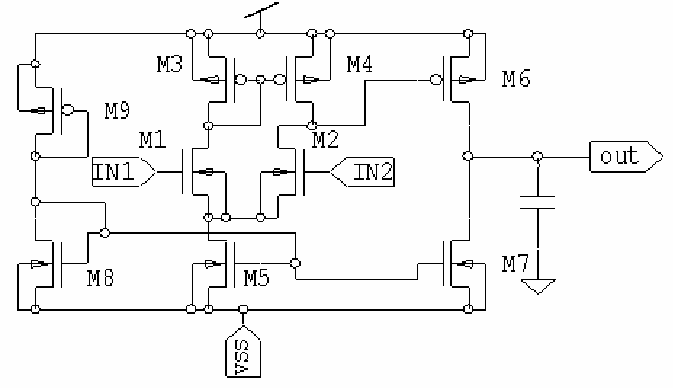
\includegraphics{CompSch.png}}
\caption{The schematic of a CMOS comparator.}
\end{figure}

\subsection{8-Bit to 3-Bit Priority Encoder}

A 8-Bit to 3-Bit Priority Encoder outputs the same as the highest order input. For the implementation in a Flash ADC, bit 0 was ignored.

An 8-Bit to 3-Bit Priority Encoder is designed in CMOS with a handful of NOT, AND, and NOR gates. Each input is either connected to an NOT gate or sent into one of the various width AND gates. The outputs of the AND gates are connected to various NOR gates. The output is each output of the NOR gates.

\begin{figure}[htbp]
\centerline{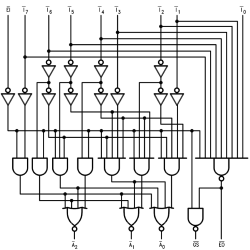
\includegraphics{PESch.png}}
\caption{The schematic of a 8-Bit to 3-Bit Priority Encoder.}
\end{figure}

\begin{table}[htbp]
\caption{8-Bit to 3-Bit Priority Encoder Truth Table}
\begin{center}
\begin{tabular}{|c|c|c|c|c|c|c|c|c|c|c|}
\hline
\multicolumn{8}{|c|}{\textbf{Input}} & \multicolumn{3}{|c|}{\textbf{Output}} \\
\hline
0 & 0 & 0 & 0 & 0 & 0 & 0 & x & 0 & 0 & 0 \\
\hline
0 & 0 & 0 & 0 & 0 & 0 & 1 & x & 0 & 0 & 1 \\
\hline
0 & 0 & 0 & 0 & 0 & 1 & 0 & x & 0 & 1 & 0 \\
\hline
0 & 0 & 0 & 0 & 0 & 1 & 1 & x & 0 & 1 & 0 \\
\hline
0 & 0 & 0 & 0 & 1 & 0 & 0 & x & 0 & 1 & 1 \\
\hline
0 & 0 & 0 & 0 & 1 & 0 & 1 & x & 0 & 1 & 1 \\
\hline
0 & 0 & 0 & 0 & 1 & 1 & 0 & x & 0 & 1 & 1 \\
\hline
0 & 0 & 0 & 0 & 1 & 1 & 1 & x & 0 & 1 & 1 \\
\hline
0 & 0 & 0 & 1 & 0 & 0 & 0 & x & 1 & 0 & 0 \\
\hline
0 & 0 & 0 & 1 & 0 & 0 & 1 & x & 1 & 0 & 0 \\
\hline
0 & 0 & 0 & 1 & 0 & 1 & 0 & x & 1 & 0 & 0 \\
\hline
0 & 0 & 0 & 1 & 0 & 1 & 1 & x & 1 & 0 & 0 \\
\hline
0 & 0 & 0 & 1 & 1 & 0 & 0 & x & 1 & 0 & 0 \\
\hline
0 & 0 & 0 & 1 & 1 & 0 & 1 & x & 1 & 0 & 0 \\
\hline
0 & 0 & 0 & 1 & 1 & 1 & 0 & x & 1 & 0 & 0 \\
\hline
0 & 0 & 0 & 1 & 1 & 1 & 1 & x & 1 & 0 & 0 \\
\hline
0 & 0 & 1 & 0 & 0 & 0 & 0 & x & 1 & 0 & 1 \\
\hline
0 & 0 & 1 & 0 & 0 & 0 & 1 & x & 1 & 0 & 1 \\
\hline
0 & 0 & 1 & 0 & 0 & 1 & 0 & x & 1 & 0 & 1 \\
\hline
0 & 0 & 1 & 0 & 0 & 1 & 1 & x & 1 & 0 & 1 \\
\hline
0 & 0 & 1 & 0 & 1 & 0 & 0 & x & 1 & 0 & 1 \\
\hline
0 & 0 & 1 & 0 & 1 & 0 & 1 & x & 1 & 0 & 1 \\
\hline
0 & 0 & 1 & 0 & 1 & 1 & 0 & x & 1 & 0 & 1 \\
\hline
0 & 0 & 1 & 0 & 1 & 1 & 1 & x & 1 & 0 & 1 \\
\hline
0 & 0 & 1 & 1 & 0 & 0 & 0 & x & 1 & 0 & 1 \\
\hline
0 & 0 & 1 & 1 & 0 & 0 & 1 & x & 1 & 0 & 1 \\
\hline
0 & 0 & 1 & 1 & 0 & 1 & 0 & x & 1 & 0 & 1 \\
\hline
0 & 0 & 1 & 1 & 0 & 1 & 1 & x & 1 & 0 & 1 \\
\hline
0 & 0 & 1 & 1 & 1 & 0 & 0 & x & 1 & 0 & 1 \\
\hline
0 & 0 & 1 & 1 & 1 & 0 & 1 & x & 1 & 0 & 1 \\
\hline
0 & 0 & 1 & 1 & 1 & 1 & 0 & x & 1 & 0 & 1 \\
\hline
0 & 0 & 1 & 1 & 1 & 1 & 1 & x & 1 & 0 & 1 \\
\hline
0 & 1 & 0 & 0 & 0 & 0 & 0 & x & 1 & 1 & 0 \\
\hline
0 & 1 & 0 & 0 & 0 & 0 & 1 & x & 1 & 1 & 0 \\
\hline
0 & 1 & 0 & 0 & 0 & 1 & 0 & x & 1 & 1 & 0 \\
\hline
0 & 1 & 0 & 0 & 0 & 1 & 1 & x & 1 & 1 & 0 \\
\hline
0 & 1 & 0 & 0 & 1 & 0 & 0 & x & 1 & 1 & 0 \\
\hline
0 & 1 & 0 & 0 & 1 & 0 & 1 & x & 1 & 1 & 0 \\
\hline
0 & 1 & 0 & 0 & 1 & 1 & 0 & x & 1 & 1 & 0 \\
\hline
0 & 1 & 0 & 0 & 1 & 1 & 1 & x & 1 & 1 & 0 \\
\hline
0 & 1 & 0 & 1 & 0 & 0 & 0 & x & 1 & 1 & 0 \\
\hline
0 & 1 & 0 & 1 & 0 & 0 & 1 & x & 1 & 1 & 0 \\
\hline
0 & 1 & 0 & 1 & 0 & 1 & 0 & x & 1 & 1 & 0 \\
\hline
0 & 1 & 0 & 1 & 0 & 1 & 1 & x & 1 & 1 & 0 \\
\hline
0 & 1 & 0 & 1 & 1 & 0 & 0 & x & 1 & 1 & 0 \\
\hline
0 & 1 & 0 & 1 & 1 & 0 & 1 & x & 1 & 1 & 0 \\
\hline
0 & 1 & 0 & 1 & 1 & 1 & 0 & x & 1 & 1 & 0 \\
\hline
0 & 1 & 0 & 1 & 1 & 1 & 1 & x & 1 & 1 & 0 \\
\hline
0 & 1 & 1 & 0 & 0 & 0 & 0 & x & 1 & 1 & 0 \\
\hline
0 & 1 & 1 & 0 & 0 & 0 & 1 & x & 1 & 1 & 0 \\
\hline
0 & 1 & 1 & 0 & 0 & 1 & 0 & x & 1 & 1 & 0 \\
\hline
0 & 1 & 1 & 0 & 0 & 1 & 1 & x & 1 & 1 & 0 \\
\hline
0 & 1 & 1 & 0 & 1 & 0 & 0 & x & 1 & 1 & 0 \\
\hline
0 & 1 & 1 & 0 & 1 & 0 & 1 & x & 1 & 1 & 0 \\
\hline
0 & 1 & 1 & 0 & 1 & 1 & 0 & x & 1 & 1 & 0 \\
\hline
0 & 1 & 1 & 0 & 1 & 1 & 1 & x & 1 & 1 & 0 \\
\hline
0 & 1 & 1 & 1 & 0 & 0 & 0 & x & 1 & 1 & 0 \\
\hline
0 & 1 & 1 & 1 & 0 & 0 & 1 & x & 1 & 1 & 0 \\
\hline
0 & 1 & 1 & 1 & 0 & 1 & 0 & x & 1 & 1 & 0 \\
\hline
0 & 1 & 1 & 1 & 0 & 1 & 1 & x & 1 & 1 & 0 \\
\hline
0 & 1 & 1 & 1 & 1 & 0 & 0 & x & 1 & 1 & 0 \\
\hline
0 & 1 & 1 & 1 & 1 & 0 & 1 & x & 1 & 1 & 0 \\
\hline
0 & 1 & 1 & 1 & 1 & 1 & 0 & x & 1 & 1 & 0 \\
\hline
0 & 1 & 1 & 1 & 1 & 1 & 1 & x & 1 & 1 & 0 \\
\hline
1 & 0 & 0 & 0 & 0 & 0 & 0 & x & 1 & 1 & 1 \\
\hline
1 & 0 & 0 & 0 & 0 & 0 & 1 & x & 1 & 1 & 1 \\
\hline
1 & 0 & 0 & 0 & 0 & 1 & 0 & x & 1 & 1 & 1 \\
\hline
1 & 0 & 0 & 0 & 0 & 1 & 1 & x & 1 & 1 & 1 \\
\hline
1 & 0 & 0 & 0 & 1 & 0 & 0 & x & 1 & 1 & 1 \\
\hline
1 & 0 & 0 & 0 & 1 & 0 & 1 & x & 1 & 1 & 1 \\
\hline
1 & 0 & 0 & 0 & 1 & 1 & 0 & x & 1 & 1 & 1 \\
\hline
1 & 0 & 0 & 0 & 1 & 1 & 1 & x & 1 & 1 & 1 \\
\hline
1 & 0 & 0 & 1 & 0 & 0 & 0 & x & 1 & 1 & 1 \\
\hline
1 & 0 & 0 & 1 & 0 & 0 & 1 & x & 1 & 1 & 1 \\
\hline
1 & 0 & 0 & 1 & 0 & 1 & 0 & x & 1 & 1 & 1 \\
\hline
1 & 0 & 0 & 1 & 0 & 1 & 1 & x & 1 & 1 & 1 \\
\hline
1 & 0 & 0 & 1 & 1 & 0 & 0 & x & 1 & 1 & 1 \\
\hline
1 & 0 & 0 & 1 & 1 & 0 & 1 & x & 1 & 1 & 1 \\
\hline
1 & 0 & 0 & 1 & 1 & 1 & 0 & x & 1 & 1 & 1 \\
\hline
1 & 0 & 0 & 1 & 1 & 1 & 1 & x & 1 & 1 & 1 \\
\hline
1 & 0 & 1 & 0 & 0 & 0 & 0 & x & 1 & 1 & 1 \\
\hline
1 & 0 & 1 & 0 & 0 & 0 & 1 & x & 1 & 1 & 1 \\
\hline
1 & 0 & 1 & 0 & 0 & 1 & 0 & x & 1 & 1 & 1 \\
\hline
1 & 0 & 1 & 0 & 0 & 1 & 1 & x & 1 & 1 & 1 \\
\hline
1 & 0 & 1 & 0 & 1 & 0 & 0 & x & 1 & 1 & 1 \\
\hline
1 & 0 & 1 & 0 & 1 & 0 & 1 & x & 1 & 1 & 1 \\
\hline
1 & 0 & 1 & 0 & 1 & 1 & 0 & x & 1 & 1 & 1 \\
\hline
1 & 0 & 1 & 0 & 1 & 1 & 1 & x & 1 & 1 & 1 \\
\hline
1 & 0 & 1 & 1 & 0 & 0 & 0 & x & 1 & 1 & 1 \\
\hline
1 & 0 & 1 & 1 & 0 & 0 & 1 & x & 1 & 1 & 1 \\
\hline
1 & 0 & 1 & 1 & 0 & 1 & 0 & x & 1 & 1 & 1 \\
\hline
1 & 0 & 1 & 1 & 0 & 1 & 1 & x & 1 & 1 & 1 \\
\hline
1 & 0 & 1 & 1 & 1 & 0 & 0 & x & 1 & 1 & 1 \\
\hline
1 & 0 & 1 & 1 & 1 & 0 & 1 & x & 1 & 1 & 1 \\
\hline
1 & 0 & 1 & 1 & 1 & 1 & 0 & x & 1 & 1 & 1 \\
\hline
1 & 0 & 1 & 1 & 1 & 1 & 1 & x & 1 & 1 & 1 \\
\hline
1 & 1 & 0 & 0 & 0 & 0 & 0 & x & 1 & 1 & 1 \\
\hline
1 & 1 & 0 & 0 & 0 & 0 & 1 & x & 1 & 1 & 1 \\
\hline
1 & 1 & 0 & 0 & 0 & 1 & 0 & x & 1 & 1 & 1 \\
\hline
1 & 1 & 0 & 0 & 0 & 1 & 1 & x & 1 & 1 & 1 \\
\hline
1 & 1 & 0 & 0 & 1 & 0 & 0 & x & 1 & 1 & 1 \\
\hline
1 & 1 & 0 & 0 & 1 & 0 & 1 & x & 1 & 1 & 1 \\
\hline
1 & 1 & 0 & 0 & 1 & 1 & 0 & x & 1 & 1 & 1 \\
\hline
1 & 1 & 0 & 0 & 1 & 1 & 1 & x & 1 & 1 & 1 \\
\hline
1 & 1 & 0 & 1 & 0 & 0 & 0 & x & 1 & 1 & 1 \\
\hline
1 & 1 & 0 & 1 & 0 & 0 & 1 & x & 1 & 1 & 1 \\
\hline
1 & 1 & 0 & 1 & 0 & 1 & 0 & x & 1 & 1 & 1 \\
\hline
1 & 1 & 0 & 1 & 0 & 1 & 1 & x & 1 & 1 & 1 \\
\hline
1 & 1 & 0 & 1 & 1 & 0 & 0 & x & 1 & 1 & 1 \\
\hline
1 & 1 & 0 & 1 & 1 & 0 & 1 & x & 1 & 1 & 1 \\
\hline
1 & 1 & 0 & 1 & 1 & 1 & 0 & x & 1 & 1 & 1 \\
\hline
1 & 1 & 0 & 1 & 1 & 1 & 1 & x & 1 & 1 & 1 \\
\hline
1 & 1 & 1 & 0 & 0 & 0 & 0 & x & 1 & 1 & 1 \\
\hline
1 & 1 & 1 & 0 & 0 & 0 & 1 & x & 1 & 1 & 1 \\
\hline
1 & 1 & 1 & 0 & 0 & 1 & 0 & x & 1 & 1 & 1 \\
\hline
1 & 1 & 1 & 0 & 0 & 1 & 1 & x & 1 & 1 & 1 \\
\hline
1 & 1 & 1 & 0 & 1 & 0 & 0 & x & 1 & 1 & 1 \\
\hline
1 & 1 & 1 & 0 & 1 & 0 & 1 & x & 1 & 1 & 1 \\
\hline
1 & 1 & 1 & 0 & 1 & 1 & 0 & x & 1 & 1 & 1 \\
\hline
1 & 1 & 1 & 0 & 1 & 1 & 1 & x & 1 & 1 & 1 \\
\hline
1 & 1 & 1 & 1 & 0 & 0 & 0 & x & 1 & 1 & 1 \\
\hline
1 & 1 & 1 & 1 & 0 & 0 & 1 & x & 1 & 1 & 1 \\
\hline
1 & 1 & 1 & 1 & 0 & 1 & 0 & x & 1 & 1 & 1 \\
\hline
1 & 1 & 1 & 1 & 0 & 1 & 1 & x & 1 & 1 & 1 \\
\hline
1 & 1 & 1 & 1 & 1 & 0 & 0 & x & 1 & 1 & 1 \\
\hline
1 & 1 & 1 & 1 & 1 & 0 & 1 & x & 1 & 1 & 1 \\
\hline
1 & 1 & 1 & 1 & 1 & 1 & 0 & x & 1 & 1 & 1 \\
\hline
1 & 1 & 1 & 1 & 1 & 1 & 1 & x & 1 & 1 & 1 \\
\hline
\end{tabular}
\end{center}
\end{table}

\subsection{Flash Analog-to-Digital Converter}

A Flash ADC uses the direct-conversion method to convert an analog signal to a digital signal.

\begin{figure}[htbp]
\centerline{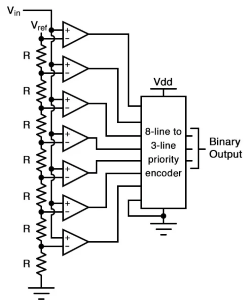
\includegraphics{ADCsch.png}}
\caption{The schematic of a 3-bit Flash ADC.}
\end{figure}

\section{Results}

All the circuits were tested for accuracy by comparing its waveforms from a testbench and accompanying truth table.

\subsection{NOT Gate}

The Testbench had a symmetrical square wave. The output perfectly mirrored the input as it should.

\subsection{Two-Input AND Gate}

The Testbench had two symmetrical square waves, one with a period twice that of the other.

\subsection{Three-Input AND Gate}

The Testbench had three symmetrical square waves, each with a period twice that of the last.

\subsection{Four-Input AND Gate}

The Testbench had three symmetrical square waves, each with a period twice that of the last.

\subsection{Four-Input NOR Gate}

The Testbench had three symmetrical square waves, each with a period twice that of the last.

\subsection{One-bit Unsigned Comparator}

The Testbench had an asymmetrical square wave that mimmicked a sawtooth wave as the VIN input. The input for VREF was a DC signal of five volts.

\subsection{8-Bit to 3-Bit Priority Encoder}

The Testbench had seven symmetrical square waves, each with a period twice that of the last.

\subsection{Flash Analog-to-Digital Converter}

The Testbench had an asymmetrical square wave that mimmicked a sawtooth wave as the VIN input. The input for VREF was a DC signal of twelve volts.

\section{Future Directions}

There are many possible future directions for a flash ADC. 
One could be To improve the power efficiency and speed of the flash ADC, different techniques such as dynamic comparator, interpolation, and folding can be researched and implemented.
Another could be to increase the resolution of the flash ADC, higher number of bits can be used. This will also increase the complexity and power consumption of the circuit.
Lastly, to try an implement a different kind of ADC, such as a Delta-Sigma ADC.

\section{Conclusions}

In this project, a 4-bit flash ADC was designed and implemented using CMOS technology in Cadence Virtuoso. The flash ADC consists of a sample and hold circuit, a resistor ladder, a set of comparators, and a priority encoder.
The main objective of the project was to achieve profiecency Cadence and its suite of applications as well as researching and implementing a particular CMOS circuit.
The results showed that the flash ADC met the design specifications.

\end{document}
